\subsection{Conception}

Nous avons développé cette application pour les systèmes d'exploitation Android. La programmation pour Android est basée sur le langage java que nous avons vu l'année dernière en cours de programmation avancée. Néanmoins, même si nous possédions de bonnes bases java, il nous a fallu plusieurs semaines afin de savoir développer sur Android car celui-ci fonctionne différemment du langage java que nous avions pu voir. \\

Une fois le langage assimilé, nous nous sommes attaqués à la conception de l'application. Nous avons tout d'abord élaboré un dessin papier des différentes vues de notre application. Au fur et à mesure que nous avancions dans le developpement nous nous sommes rendu compte qu'il serait plus compliqué que prévu de réaliser toutes ces vues. Nous avons donc opté pour une application plus simple mais qui répond à nos attentes.\\

La figure ci-dessous présente le menu de démarrage de l'application : 
	\begin{figure}[H]
		\centering
		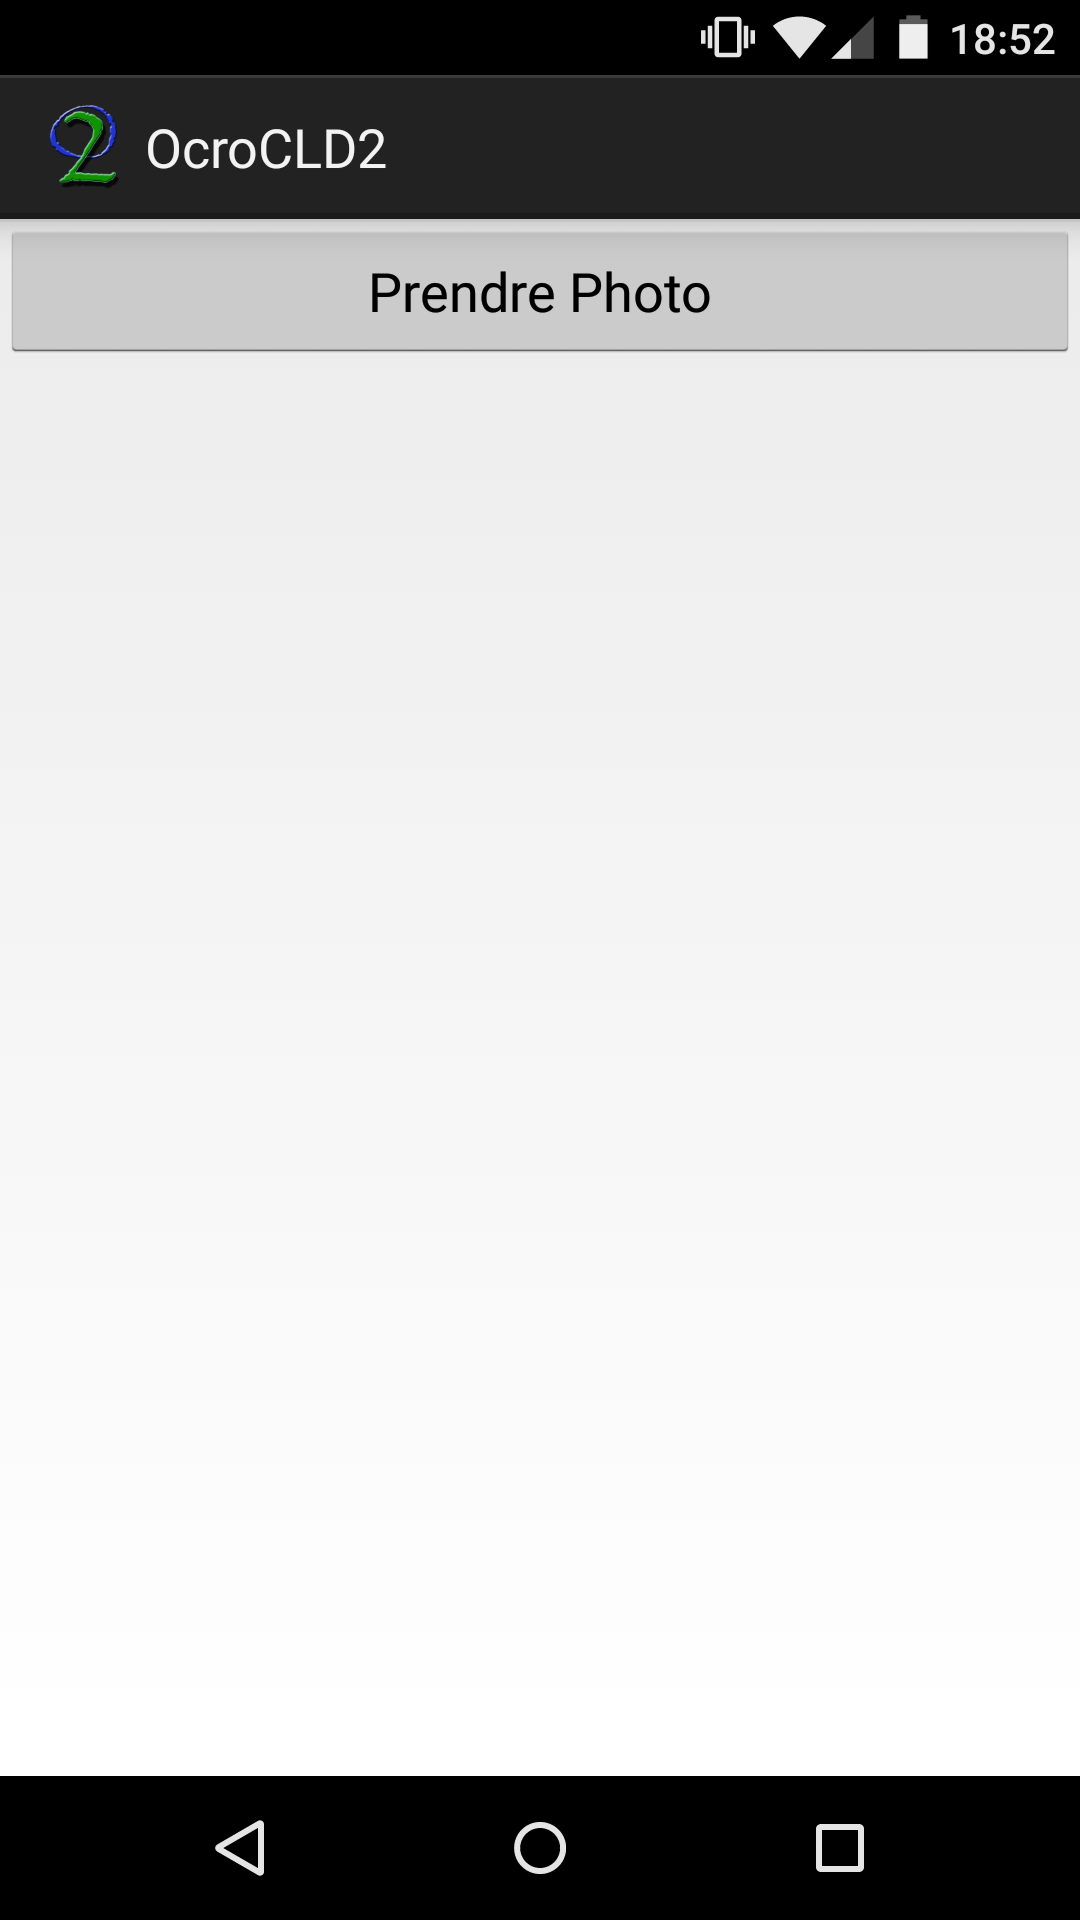
\includegraphics[scale=0.1]{images/appliMenu.png}
		\caption{Menu principal}
		\label{fig:image}
	\end{figure}

\subsection{Installation}
Pour installer l'application sur mobile Android, il suffit juste de copier ocroCLD2.apk sur le smartphone. Ensuite, activer l'installation d'applications non certifiées et installer l'application.

\subsection{Fonctionnement}
L'intégralité du code de l'application est disponible dans l'archive fournie.\\

Lorsque nous sommes dans le menu principal, il nous suffit d'appuyer sur le bouton "prendre une photo" afin que l'application fasse appel à l'application appareil photo de notre mobile. Pour faire ceci, nous utilisons un listener qui lorsque l'on clique sur le bouton, l'application crée un intent afin d'utiliser l'application en charge des photos. Ceci nous a permis de ne pas redévelopper l'appareil photo déjà présent.\\

Une fois que nous avons pris la photo, il nous suffit de valider et nous retournons à l'accueil. L'application envoie alors grâce à notre classe DataSender l'image par protocole Http sur l'adresse du script php de notre serveur. Une fois cela fait, l'application reste à l'écoute du serveur afin de récupérer la chaîne de caractère renvoyée. Cette chaîne contient le résultat du traitement par Ocropus puis CLD2.\\

Nous pouvons alors reprendre une photo ou bien quitter l'application.

\subsection{Tests}
Nous avons effectué quelques tests sur notre application dont voici l'un des résultats :
	\begin{figure}[H]
		\centering
		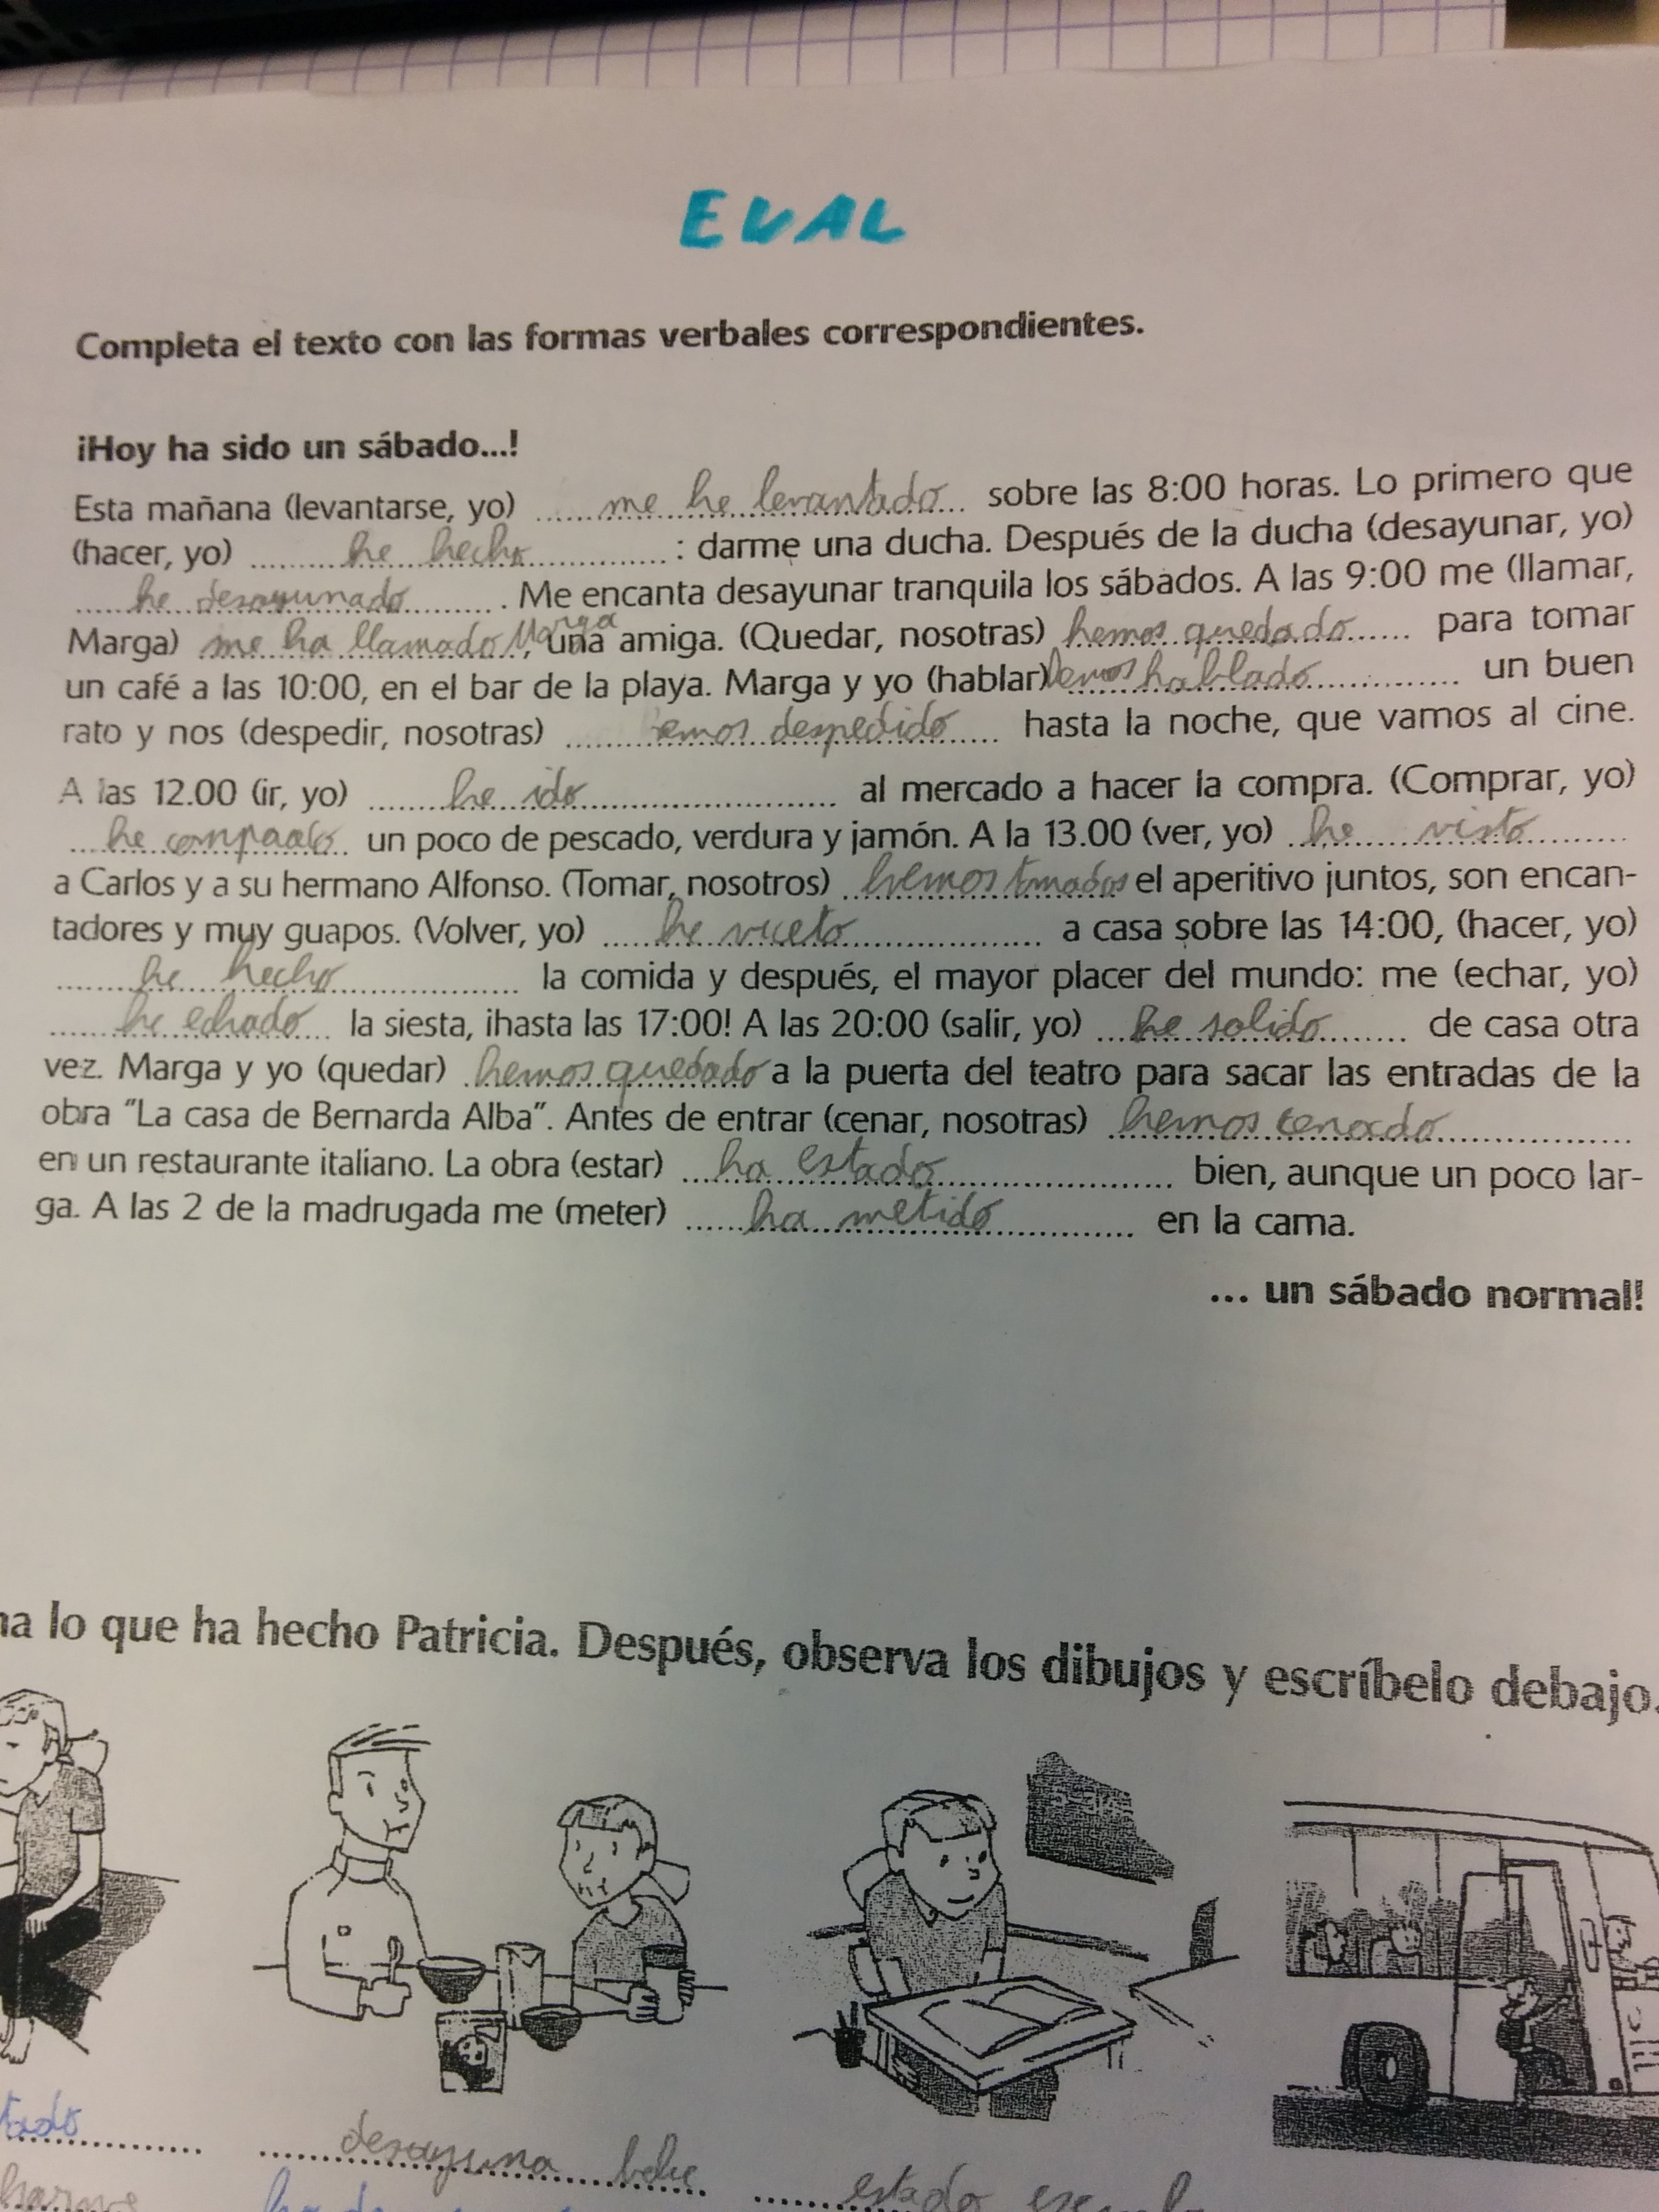
\includegraphics[scale=0.08]{images/testsImg.jpg}
		\caption{Document en espagnol pris en photo}
		\label{fig:image}
	\end{figure}
	
	\begin{figure}[H]
		\centering
		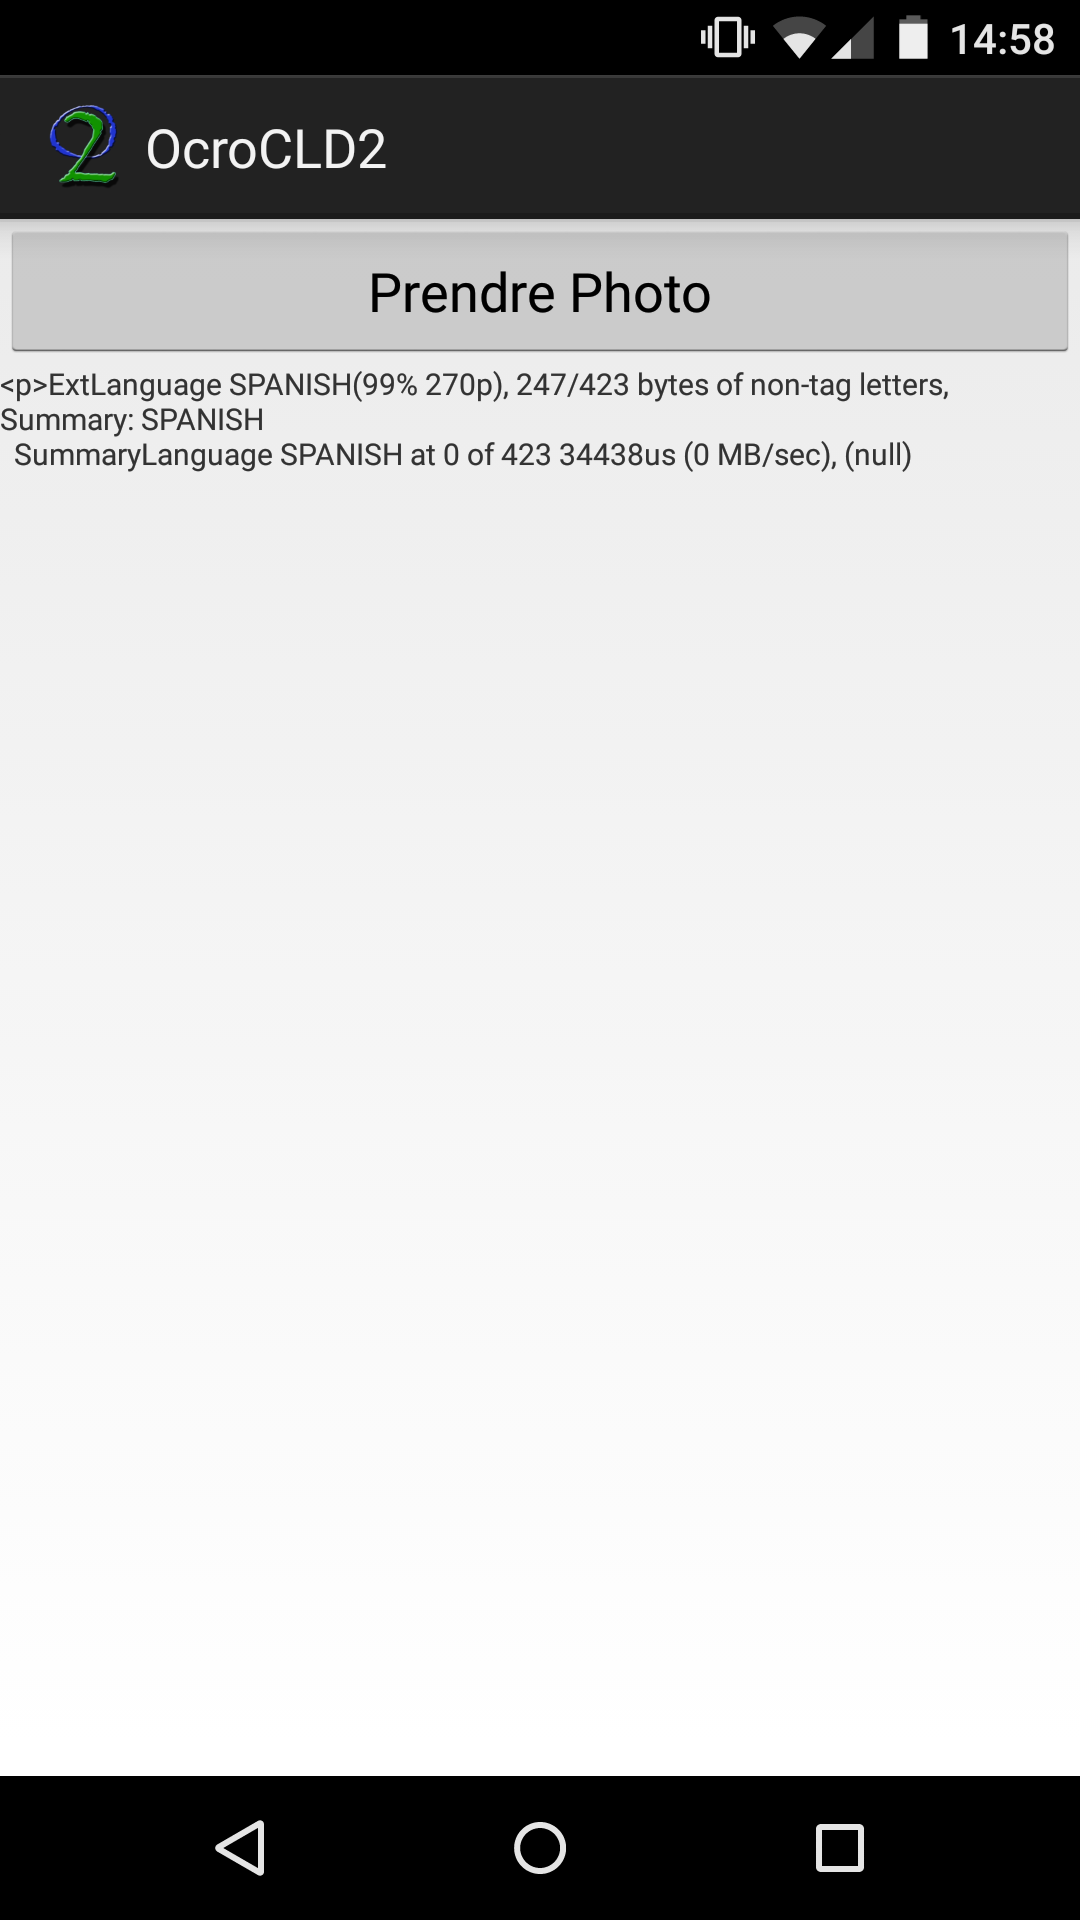
\includegraphics[scale=0.2]{images/testRes.png}
		\caption{Menu principal}
		\label{fig:image}
	\end{figure}
Nous pouvons voir que l'image a bien été traitée par le serveur et que la langue renvoyée par CLD2 est la bonne.

\subsection{Problèmes rencontrés}

Tout d'abord, l'apprentissage du java pour Android est apparu plus difficile que prévu car nous ne pensions pas qu'il y avait autant de différences. De plus, nous avons eu quelques soucis pour installer le SDK android sur Eclipse. C'est pourquoi nous avons pris un peu de retard au début de ce projet.\\

Ensuite, il a été assez compliqué de faire communiquer l'application avec le serveur. Plus précisément, nous ne savions pas quel type de protocole était le plus adapté afin d'envoyer une photo sur un serveur. Après avoir consulté Mr Nicolas Malandin, nous avons donc opté pour le protocole Http.\\

Finalement, nous avons toujours des problèmes de réponse du serveur : par moment nous ne sommes pas certain de recevoir une réponse. En effet, le traitement de l'image par Ocropus prend plusieurs minutes suivant la taille du texte à traiter.